
\documentclass{report}\usepackage[]{graphicx}\usepackage[]{color}
%% maxwidth is the original width if it is less than linewidth
%% otherwise use linewidth (to make sure the graphics do not exceed the margin)
\makeatletter
\def\maxwidth{ %
  \ifdim\Gin@nat@width>\linewidth
    \linewidth
  \else
    \Gin@nat@width
  \fi
}
\makeatother

\definecolor{fgcolor}{rgb}{0.345, 0.345, 0.345}
\newcommand{\hlnum}[1]{\textcolor[rgb]{0.686,0.059,0.569}{#1}}%
\newcommand{\hlstr}[1]{\textcolor[rgb]{0.192,0.494,0.8}{#1}}%
\newcommand{\hlcom}[1]{\textcolor[rgb]{0.678,0.584,0.686}{\textit{#1}}}%
\newcommand{\hlopt}[1]{\textcolor[rgb]{0,0,0}{#1}}%
\newcommand{\hlstd}[1]{\textcolor[rgb]{0.345,0.345,0.345}{#1}}%
\newcommand{\hlkwa}[1]{\textcolor[rgb]{0.161,0.373,0.58}{\textbf{#1}}}%
\newcommand{\hlkwb}[1]{\textcolor[rgb]{0.69,0.353,0.396}{#1}}%
\newcommand{\hlkwc}[1]{\textcolor[rgb]{0.333,0.667,0.333}{#1}}%
\newcommand{\hlkwd}[1]{\textcolor[rgb]{0.737,0.353,0.396}{\textbf{#1}}}%
\let\hlipl\hlkwb

\usepackage{framed}
\makeatletter
\newenvironment{kframe}{%
 \def\at@end@of@kframe{}%
 \ifinner\ifhmode%
  \def\at@end@of@kframe{\end{minipage}}%
  \begin{minipage}{\columnwidth}%
 \fi\fi%
 \def\FrameCommand##1{\hskip\@totalleftmargin \hskip-\fboxsep
 \colorbox{shadecolor}{##1}\hskip-\fboxsep
     % There is no \\@totalrightmargin, so:
     \hskip-\linewidth \hskip-\@totalleftmargin \hskip\columnwidth}%
 \MakeFramed {\advance\hsize-\width
   \@totalleftmargin\z@ \linewidth\hsize
   \@setminipage}}%
 {\par\unskip\endMakeFramed%
 \at@end@of@kframe}
\makeatother

\definecolor{shadecolor}{rgb}{.97, .97, .97}
\definecolor{messagecolor}{rgb}{0, 0, 0}
\definecolor{warningcolor}{rgb}{1, 0, 1}
\definecolor{errorcolor}{rgb}{1, 0, 0}
\newenvironment{knitrout}{}{} % an empty environment to be redefined in TeX

\usepackage{alltt}

\usepackage{longtable}
\usepackage[vcentering,dvips]{geometry}
\usepackage{pdflscape}
\usepackage{graphicx}
\usepackage[colorlinks = true,linkcolor = blue ]{hyperref}
\usepackage{textcomp}
\usepackage[T1]{fontenc}
\usepackage{lmodern}
\usepackage{booktabs}
\usepackage{amsmath}

\usepackage[english]{babel}
\usepackage{blindtext}

\usepackage{rotating}
\usepackage{pdflscape}



\newcommand{\HRule}{\rule{\linewidth}{0.5mm}}
\setlength{\parindent}{.3in}
\setcounter{secnumdepth}{5}
\geometry{
        letterpaper,
        left   =  1.0in,
        right  = 1.0in,
        top    = 1.0in,
        bottom = 1.0in}
\IfFileExists{upquote.sty}{\usepackage{upquote}}{}
\begin{document}


\begin{titlepage}

\begin{minipage}{0.45\textwidth}
\begin{flushleft}

\includegraphics[width=0.7\textwidth]{./source/shclogo}   
\end{flushleft}
\end{minipage}


\begin{center}




\vspace{4cm}

\textsc{\Large Data Analysis and Modeling Report }\\[0.5cm]


% Title
\HRule \\[0.4cm]
{ \huge \bfseries EGP Bounce Model}\\[0.4cm]

\HRule \\[1.5cm]

% Vendor and Client
\begin{minipage}{0.4\textwidth}
\begin{flushleft} \large
\emph{Prepared by:}\\
\textsc{Jim Crozier}
\end{flushleft}
\end{minipage}
\begin{minipage}{0.4\textwidth}
\begin{flushright} \large
\emph{Client:} \\
\textsc{MailChimp Data Science}
\end{flushright}
\end{minipage}

\vfill

% Bottom of the page
\large {Version 1}\\
{\large \today}

\end{center}

\end{titlepage}
\tableofcontents
\newpage


\section{Overview}
Example text
\begin{itemize}
  \item Move data into Hive and Spark from Postgres + R 
  \item Generate dependent variable and feature set 
  \item Fit models and test for accuracy
  \begin{itemize}
  \item Test LM, Logitistic, Random Forest, Gradient Descent 
  \item Test using all data vs history and no-history
  \item Test variety of feature sets
  \end{itemize}
\end{itemize}

\newpage 

\section{Exploratory Data Analysis}


\subsection{Sends Data}
The raw dataset included limited data from May of 2016 to July of 2017...
\begin{kframe}


{\ttfamily\noindent\color{warningcolor}{\#\# Warning: Removed 20 rows containing missing values (geom\_path).}}\end{kframe}


For the analytical dataset I cut the data down to July, 2016 - April, 2017

\begin{kframe}


{\ttfamily\noindent\color{warningcolor}{\#\# Warning: Removed 20 rows containing missing values (geom\_path).}}

{\ttfamily\noindent\color{warningcolor}{\#\# Warning: Removed 20 rows containing missing values (geom\_path).}}\end{kframe}
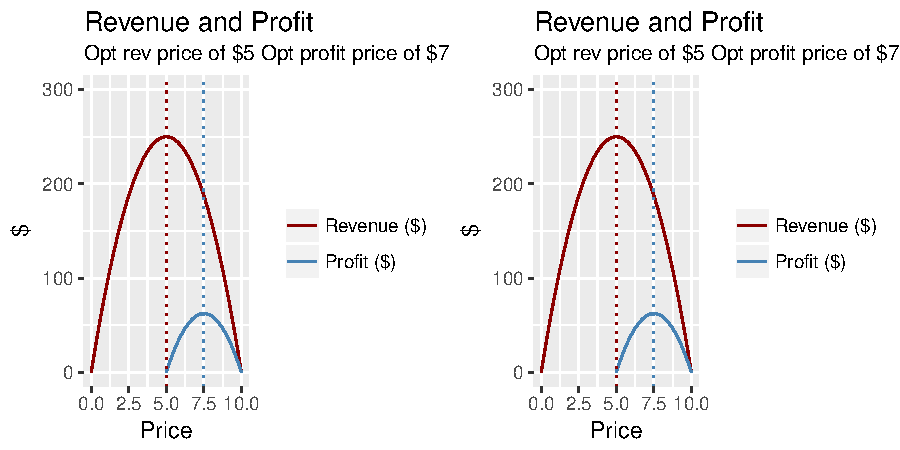
\includegraphics[width=\maxwidth]{figure/unnamed-chunk-2-1} 



\section{Analytical Dataset}

\subsection{Dependent Variable}




\subsubsection{Some subsection }


% latex table generated in R 3.4.2 by xtable 1.8-2 package
% Sat Jan  6 14:33:41 2018
\begin{table}[ht]
\centering
\caption{Top Line Domain} 
\begin{tabular}{rrrrr}
  \hline
 & q & p & rev & profit \\ 
  \hline
1 & 100.00 & 0.00 & 0.00 & -500.00 \\ 
  2 & 90.00 & 1.00 & 90.00 & -360.00 \\ 
  3 & 80.00 & 2.00 & 160.00 & -240.00 \\ 
  4 & 70.00 & 3.00 & 210.00 & -140.00 \\ 
  5 & 60.00 & 4.00 & 240.00 & -60.00 \\ 
  6 & 50.00 & 5.00 & 250.00 & 0.00 \\ 
  7 & 40.00 & 6.00 & 240.00 & 40.00 \\ 
  8 & 30.00 & 7.00 & 210.00 & 60.00 \\ 
  9 & 20.00 & 8.00 & 160.00 & 60.00 \\ 
  10 & 10.00 & 9.00 & 90.00 & 40.00 \\ 
  11 & 0.00 & 10.00 & 0.00 & 0.00 \\ 
   \hline
\end{tabular}
\end{table}

               
                             
\subsection{Model}
\begin{equation}
  \operatorname{Pr}(\text{Event} = 1 \mid \text{X})
 = \frac{\exp(\beta_{0} + \beta_{1} \text{Gender} + \beta_{2} \text{Age} + \dots +
    \beta_{12} \text{immigration)} }{1 + \exp(\beta_{0} + \beta_{1} \text{Gender} + \beta_{2} \text{Age} +
\dots + \beta_{12 }\text{immigration})} \label{eq:glm1} 
\end{equation}

\subsection{Some Subsection}


\blindtext

\begin{figure}[ !htb]
\minipage{0.49\textwidth}
  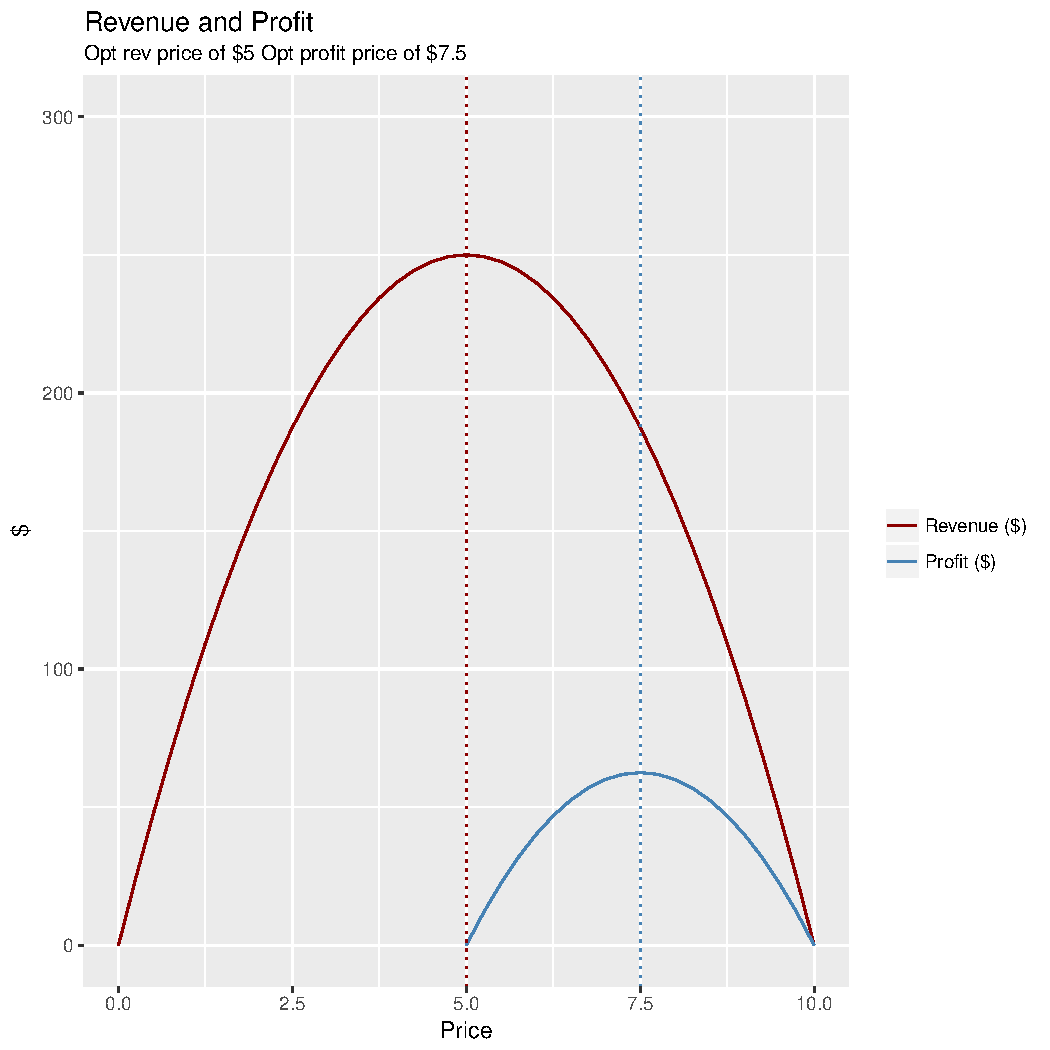
\includegraphics[width=\linewidth,height = 6cm]{optprice.pdf}
  \caption{Model 1 Importance}\label{fig:awesome_image1}
\endminipage\hfill
\minipage{0.49\textwidth}
  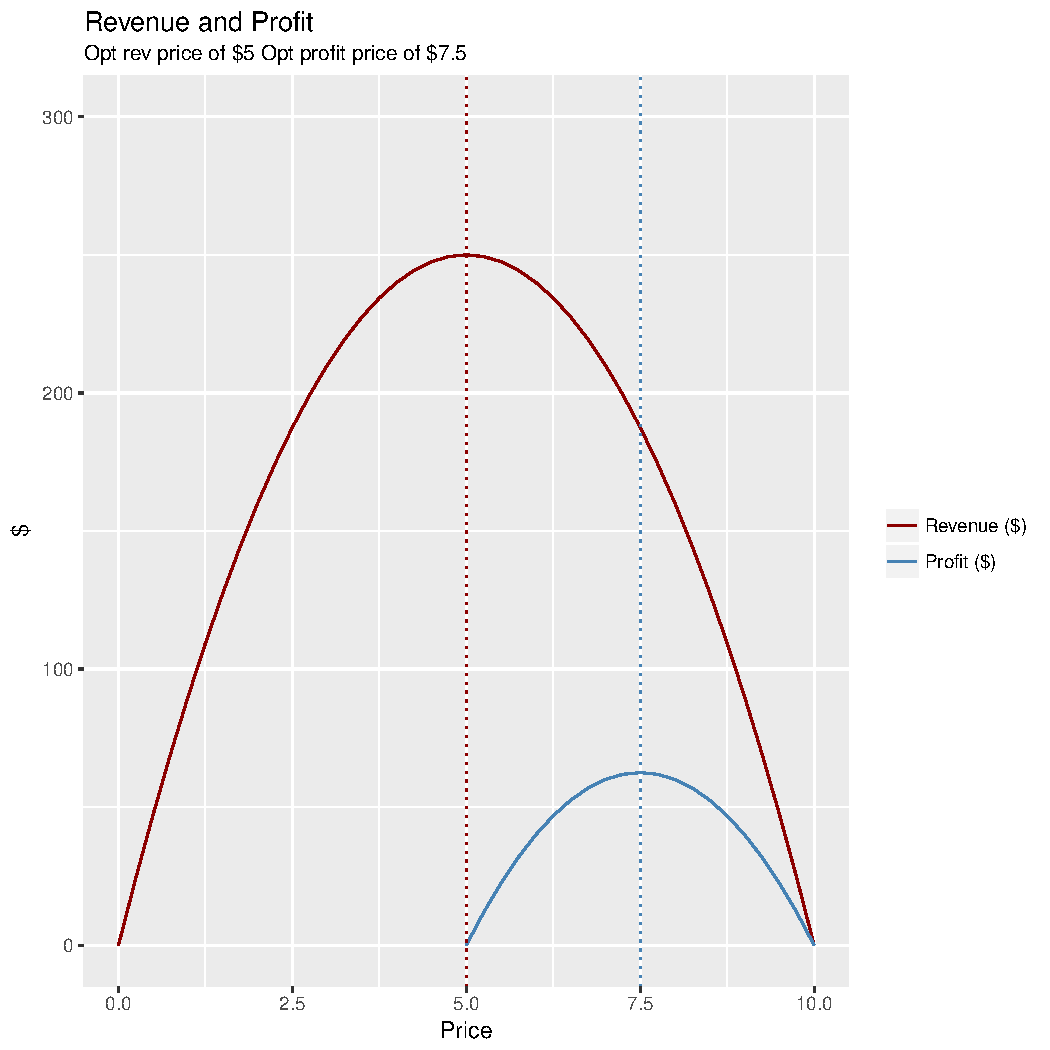
\includegraphics[width=\linewidth]{optprice.pdf}
  \caption{Model 1 Effects}\label{fig:awesome_image2}
\endminipage\hfill

\end{figure}


\blindtext

\end{document}
